\section{Description et analyse d'une entreprise atypique: \\Probespoke}
\subsection{ProBespoke une entreprise innovante}

\paragraph{Histoire de l'entreprise}
Probespoke a été fondée en 2012. Il s'agissait tout d'abord de réunir les différentes usines textiles de Bangkok.
Une plateforme informatique commune devais permettre la distribution des commandes venant d'Europe et d'Amérique du Nord.
Mais une différence de point vus à fait éclater le projet. Un des fondateurs, Christophe Saska décida de reprendre le projet sous une forme différente. Il finalisa avec l'aide d'une équipe d'informaticiens la plateforme et devellopa une application distribuée aux tailleurs pour prendre les commandes. Il agit donc comme un \textit{trader} entre des tailleurs, principalement européeens et américains et les usines thailandaises.(voir Figure 1)
\paragraph{}
\begin{figure}[h]
\begin{tikzpicture}[node distance=1cm, auto]
\tikzset{
    mynode/.style={rectangle,rounded corners,draw=black, top color=white, bottom color=yellow!50,very thick, inner sep=1em, minimum size=3em, text centered},
    mynodevert/.style={rectangle,rounded corners,draw=black, top color=white, bottom color=green!50,very thick, inner sep=1em, minimum size=3em, text centered},
    myarrow/.style={->, >=latex', shorten >=1pt, thick},
    myarrowargent/.style={->, >=latex', shorten >=1pt, thick,color=red},
    mylabel/.style={text width=7em, text centered}
}
\node[mynode] (client) {Clients finaux};
\node[mynode, right=2cm of client] (tailleur) {Tailleurs};
\node[mynode, right=2cm of tailleur] (probespoke) {Probespoke};
\node[mynode,right=2cm of probespoke] (atelier) {Atelier};

\node[mynodevert,below=2cm of tailleur] (app) {Application};
\node[mynodevert,below=2cm of probespoke] (serveur) {Serveur};

\draw[->, >=latex', shorten >=2pt, shorten <=2pt, bend right=45, thick, dashed]
    (atelier.north) to node[auto, swap] {Costume}(probespoke.north);
\draw[->, >=latex', shorten >=2pt, shorten <=2pt, bend right=45, thick, dashed]
    (probespoke.north) to node[auto, swap] {Costume vérifié}(tailleur.north);
\draw[->, >=latex', shorten >=2pt, shorten <=2pt, bend right=45, thick, dashed]
    (tailleur.north) to node[auto, swap] {Présente le costume au client}(client.north);

\draw[myarrow] (tailleur.south) to node[auto,swap] {Commande}  (app.north);
\draw[myarrow] (probespoke.south) to node[auto,swap] {Contrôle}  (serveur.north);
\draw[myarrow] (app.east) to node[auto,swap] {Transmet}  (serveur.west);
\draw[myarrow] (serveur.east) to node[auto,swap] {Imprime la commande}  (atelier.south);

\draw[myarrowargent] (client.east) to node[auto,swap] {paye} (tailleur.west);
\draw[myarrowargent] (tailleur.east) to node[auto,swap] {paye}  (probespoke.west);
\draw[myarrowargent] (probespoke.east) to node[auto,swap] {paye}  (atelier.west);

\end{tikzpicture}
\medskip
\caption{Workflow de l'entreprise Probespoke}
\end{figure}

\paragraph{}
\clearpage
\begin{wrapfigure}[12]{o}{8cm}
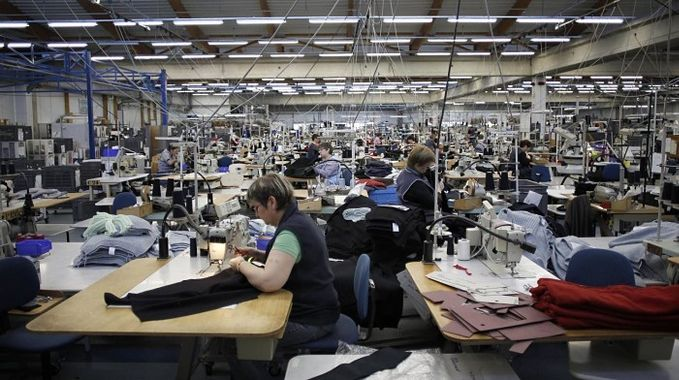
\includegraphics[width=8cm]{image/textile.jpg}
\caption{Une usine textile}
\end{wrapfigure}
\paragraph{Justification de l'existence}
 La fabrication d'une pièce sur mesure est décomposée sur plusieurs postes sur la chaine d'assemblage. Une équipe ne s'occupe que des manches, une autre que des poches, et ainsi de suite. Ces équipes ont besoin d'être formées par des maîtres tailleurs expérimentés afin de correspondre aux attentes qualités du client. Cette charge de travail est difficile à supporter pour des tailleurs occidentaux peu habitués aux façons de travailler en Thailande. Du côté des ateliers thailandais, cet intermédiare leur permet de ne pas avoir à s'occuper du démarchage des clients. Il s'agit donc d'une opportunité pour tout le monde.
